% !TEX TS-program = pdflatex
% !TEX encoding = UTF-8 Unicode

\documentclass{beamer}
\setbeamercovered{invisible}

\mode<presentation>
{
  \usetheme{Warsaw}
}

\usepackage[english]{babel}
\usepackage[utf8]{inputenc}
\usepackage{times}
\usepackage[T1]{fontenc}
\usepackage{tikz}
\usepackage{amsmath}

\title{MATH 180 Strategies of Problem Solving}
\subtitle{}
\author[W.R. Casper]{W.R. Casper}
\institute[California State University Fullerton]
{
  Department of Mathematics\\
  California State University Fullerton
}
\date{September 9, 2026}
\subject{Talks}

% Suggested timing: 110 minutes total, including a 5-minute coffee break.
%   0--5      Opening question
%   5--17     Count 3-by-4 Chomp boards in groups
%   17--28    Row lengths and Young diagrams
%   28--41    Boundary-path correspondence
%   41--52    Multiplication principle and factorials
%   52--57    Coffee break
%   57--70    Repeated objects and the binomial formula
%   70--83    Binomial coefficient examples and identities
%   83--91    General m-by-n board formula
%   91--104   Real-world application activity and discussion
%   104--110  Question of the Day and reflection

% Chomp orientation: row lengths are listed bottom-to-top.
% The poisoned square remains in the bottom-left.
\newcommand{\chompdiagram}[1]{%
  \begin{tikzpicture}[scale=.48,baseline=(current bounding box.center)]
    \foreach \len [count=\r from 0] in {#1}{
      \foreach \c in {1,...,\len}{
        \draw[fill=brown!15] ({\c-1},\r) rectangle (\c,{\r+1});
      }
    }
    \fill[green!35] (0,0) rectangle (1,1);
    \draw (0,0) rectangle (1,1);
    \node[font=\scriptsize\bfseries] at (.5,.5) {P};
  \end{tikzpicture}%
}

\AtBeginSubsection[]
{
  \begin{frame}<beamer>{Outline}
    \tableofcontents[currentsection,currentsubsection]
  \end{frame}
}

\begin{document}

\begin{frame}
  \titlepage
\end{frame}

\begin{frame}{Outline}
  \tableofcontents
\end{frame}

\section{Board Shapes}
\subsection{Young Diagrams}

\begin{frame}{Question from last time}
\pause
  \begin{block}{Puzzle}
    Start with a $3\times4$ Chomp board.
    How many different board shapes can occur during play?
    \begin{center}
      \chompdiagram{4,4,4}
    \end{center}
  \end{block}
\pause
  \begin{block}{A detail to decide}
    Should we include the empty board after someone eats the poison?
  \end{block}
\end{frame}

\begin{frame}{Counting board shapes}
  \begin{block}{Activity (10 mins)}
    Work with your neighbors.
    \begin{itemize}
      \item Find a systematic way to describe every possible shape.
      \item Count without repeating a shape.
      \item Explain how you know your list is complete.
    \end{itemize}
  \end{block}
\pause
  \begin{block}{A useful goal}
    Replace the pictures with objects that are easier to count.
  \end{block}
\end{frame}

\begin{frame}{Some possible boards}
  \begin{center}
    \chompdiagram{4,4,4}
    \qquad
    \chompdiagram{4,3,1}
    \qquad
    \chompdiagram{3,2,2}
    \qquad
    \chompdiagram{2,1,1}
  \end{center}
\pause
  \begin{block}{Question}
    How could we describe each board without drawing it?
  \end{block}
\end{frame}

\begin{frame}{Row lengths}
  \begin{block}{Encoding}
    Read the row lengths from bottom to top.
    \begin{center}
      \chompdiagram{4,3,1}
      \qquad corresponds to \qquad
      $(4,3,1)$.
    \end{center}
  \end{block}
\pause
  \begin{block}{Question}
    Which triples $(a,b,c)$ describe possible boards inside a
    $3\times4$ rectangle?
  \end{block}
\end{frame}

\begin{frame}{The condition on the rows}
  \begin{block}{Answer}
    A board inside a $3\times4$ rectangle has row lengths
    \[
       4\geq a\geq b\geq c\geq0.
    \]
  \end{block}
\pause
  \begin{block}{Reason}
    A square cannot remain unless every square below it and every
    square to its left also remains.
  \end{block}
\pause
  \begin{block}{Terminology}
    Mathematicians call a shape of left-aligned rows with decreasing
    lengths a \textbf{Young diagram}.
  \end{block}
\end{frame}

\begin{frame}{Young diagrams in our orientation}
\small
  \begin{block}{Usual convention}
    Young diagrams are often drawn with the longest row on top.
  \end{block}
\pause
  \begin{block}{Our convention}
    We draw the longest row on the bottom so the poisoned square stays
    in the bottom-left, just as it did in Chomp.
  \end{block}
\pause
  \begin{block}{Same mathematical object}
    Turning the paper upside down changes the picture, but not the row
    lengths or the counting problem.
  \end{block}
\end{frame}

\begin{frame}{A first census}
  \begin{block}{Warm-up}
    How many Young diagrams fit inside each rectangle?
  \end{block}
  \begin{center}
    \begin{tabular}{c|c|c|c}
      Rectangle & $1\times n$ & $2\times2$ & $2\times3$ \\
      \hline
      Number of shapes & ? & ? & ?
    \end{tabular}
  \end{center}
\pause
  \begin{block}{Answers}
    \[
      n+1, \qquad 6, \qquad 10.
    \]
  \end{block}
\pause
  \begin{block}{Question}
    What pattern might continue?
  \end{block}
\end{frame}

\subsection{Boundary Paths}

\begin{frame}{A path around every shape}
\small
  \begin{block}{Boundary idea}
    Trace the boundary separating the remaining chocolate from the
    missing chocolate.
  \end{block}
\pause
  \begin{center}
    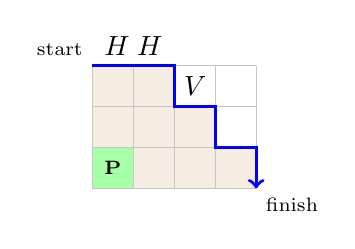
\begin{tikzpicture}[scale=.52]
      \foreach \x in {0,...,3}{
        \fill[brown!15] (\x,0) rectangle ({\x+1},1);
      }
      \foreach \x in {0,...,2}{
        \fill[brown!15] (\x,1) rectangle ({\x+1},2);
      }
      \foreach \x in {0,...,1}{
        \fill[brown!15] (\x,2) rectangle ({\x+1},3);
      }
      \fill[green!35] (0,0) rectangle (1,1);
      \draw[step=1cm,gray!45,thin] (0,0) grid (4,3);
      \draw[blue,very thick,->]
        (0,3)--(1,3)--(2,3)--(2,2)--(3,2)--(3,1)--(4,1)--(4,0);
      \node[above] at (1,3) {$H\;H$};
      \node[right] at (2,2.5) {$V$};
      \node[font=\scriptsize,above left] at (0,3) {start};
      \node[font=\scriptsize,below right] at (4,0) {finish};
      \node[font=\scriptsize\bfseries] at (.5,.5) {P};
    \end{tikzpicture}
  \end{center}
\pause
  \begin{block}{$3\times4$ rectangle}
    Every boundary uses four horizontal steps and three vertical steps.
  \end{block}
\end{frame}

\begin{frame}{From paths to words}
  \begin{block}{Record each step}
    Read from top-left to bottom-right.  Write $H$ for a step to the right
    and $V$ for a step downward.
  \end{block}
\pause
  \begin{block}{Example}
    \[
       HHVHVHV
    \]
  \end{block}
\pause
  \begin{block}{What every word contains}
    Exactly four $H$'s and three $V$'s, in some order.
  \end{block}
\end{frame}

\begin{frame}{Why this correspondence works}
\small
  \begin{block}{Young diagram to word}
    Each Young diagram has one boundary path, so it produces one word.
  \end{block}
\pause
  \begin{block}{Word to Young diagram}
    A word with four $H$'s and three $V$'s traces one path across the
    rectangle.  The squares on the bottom-left side form one Young diagram.
  \end{block}
\pause
  \begin{block}{Bijection}
    Every diagram gets one word, and every word gets one diagram.
    Therefore the two collections have the same size.
  \end{block}
\end{frame}

\begin{frame}{The counting problem has changed}
\small
  \begin{block}{Original question}
    How many Young diagrams fit in a $3\times4$ rectangle?
  \end{block}
\pause
  \begin{block}{Equivalent question}
    How many different arrangements of
    \[
       H,H,H,H,V,V,V
    \]
    are possible?
  \end{block}
\pause
  \begin{block}{Strategy}
    We first learn to count arrangements of objects that are all different.
  \end{block}
\end{frame}

\section{Counting Tools}
\subsection{Factorials}

\begin{frame}{The multiplication principle}
\small
  \begin{block}{Two consecutive choices}
    If a first choice has $a$ possibilities and each can be followed by
    $b$ possibilities, then the pair of choices has $ab$ possibilities.
  \end{block}
\pause
  \begin{block}{Example}
    Three shirts and four pairs of pants make
    \[
       3\cdot4=12
    \]
    possible outfits.
  \end{block}
\pause
  \begin{block}{More than two choices}
    Multiply the number of possibilities at each stage.
  \end{block}
\end{frame}

\begin{frame}{Arranging different objects}
  \begin{block}{Example}
    Four students will give presentations.  How many speaking orders are possible?
  \end{block}
\pause
  \begin{block}{Fill the four positions}
    \[
      \underbrace{4}_{\text{first}}
      \cdot
      \underbrace{3}_{\text{second}}
      \cdot
      \underbrace{2}_{\text{third}}
      \cdot
      \underbrace{1}_{\text{fourth}}
      =24.
    \]
  \end{block}
\pause
  \begin{block}{Why the numbers decrease}
    Once a student has a position, that student cannot be chosen again.
  \end{block}
\end{frame}

\begin{frame}{Factorials}
\footnotesize
  \begin{block}{Definition}
    For a positive integer $n$,
    \[
       n!=n(n-1)(n-2)\cdots2\cdot1.
    \]
  \end{block}
\pause
  \begin{block}{Meaning}
    $n!$ counts the orders of $n$ different objects.
  \end{block}
\pause
  \begin{block}{Examples}
    \[
      3!=6,\qquad 5!=120,\qquad 7!=5040.
    \]
  \end{block}
\pause
  \begin{block}{Useful convention}
    $0!=1$: there is exactly one way to arrange no objects, the empty order.
  \end{block}
\end{frame}

\begin{frame}{A factorial checkpoint}
  \begin{block}{Think, then compare}
    Seven different books are placed in a row.
    \begin{enumerate}
      \item How many orders are possible?
      \item How many orders put a particular book first?
      \item How many orders put two particular books next to each other?
    \end{enumerate}
  \end{block}
\pause
  \begin{block}{Answers}
    \[
       7!,\qquad 6!,\qquad 2\cdot6!.
    \]
  \end{block}
\end{frame}

\begin{frame}{Coffee break (5 mins)}
  \begin{center}
    \Large
    Why is $7!$ too large for arranging\\[.75em]
    \[
       H,H,H,H,V,V,V\,?
    \]
  \end{center}
\end{frame}

\subsection{Binomial Coefficients}

\begin{frame}{Repeated objects change the count}
\footnotesize
  \begin{block}{Pretend the letters have labels}
    Arrange
    \[
      H_1,H_2,H_3,H_4,V_1,V_2,V_3.
    \]
    Since these seven objects are different, there are $7!$ orders.
  \end{block}
\pause
  \begin{block}{Erase the labels}
    Every visible $H/V$ word came from
    \[
       4!\cdot3!
    \]
    labeled orders: the $H$ labels and $V$ labels can be rearranged invisibly.
\pause
    Therefore the corrected count is
    \[
       \frac{7!}{4!3!}=35.
    \]
  \end{block}
\end{frame}

\begin{frame}{A second route: choose positions}
  \begin{block}{Seven empty positions}
    \[
       \_\quad\_\quad\_\quad\_\quad\_\quad\_\quad\_
    \]
  \end{block}
\pause
  \begin{block}{Choose three positions for $V$}
    Once those positions are chosen, all four remaining positions must contain $H$.
  \end{block}
\pause
  \begin{block}{Same question}
    How many ways can we choose three positions from seven positions?
  \end{block}
\end{frame}

\begin{frame}{Binomial coefficients}
\small
  \begin{block}{Notation}
    Read $\binom{n}{k}$ as ``$n$ choose $k$.''
  \end{block}
\pause
  \begin{block}{Meaning}
    $\binom{n}{k}$ counts ways to choose $k$ objects from $n$ different objects
    when the order of the chosen objects does not matter.
  \end{block}
\pause
  \begin{block}{Formula}
    \[
       \boxed{\binom{n}{k}=\frac{n!}{k!(n-k)!}}.
    \]
  \end{block}
\end{frame}

\begin{frame}{Why the binomial formula works}
\small
  \begin{block}{First count ordered selections}
    Choose $k$ objects in order:
    \[
       n(n-1)\cdots(n-k+1)=\frac{n!}{(n-k)!}.
    \]
  \end{block}
\pause
  \begin{block}{Then forget the order}
    Each group of $k$ objects appears in $k!$ different orders.
  \end{block}
\pause
  \begin{block}{Divide out the overcount}
    \[
       \binom{n}{k}
       =\frac{n!}{(n-k)!}\cdot\frac{1}{k!}
       =\frac{n!}{k!(n-k)!}.
    \]
  \end{block}
\end{frame}

\begin{frame}{Example: choosing a committee}
  \begin{block}{Problem}
    A class has eight students.  How many three-student committees are possible?
  \end{block}
\pause
  \begin{block}{Calculation}
    \[
      \binom{8}{3}=\frac{8!}{3!5!}
      =\frac{8\cdot7\cdot6}{3\cdot2\cdot1}=56.
    \]
  \end{block}
\pause
  \begin{block}{Important distinction}
    A committee has no first, second, or third position.  If the jobs were
    different, we would count an ordered selection instead.
  \end{block}
\end{frame}

\begin{frame}{Example: binary messages}
\footnotesize
  \begin{block}{Problem}
    How many eight-bit messages contain exactly three $1$'s?
  \end{block}
\pause
  \begin{block}{Choose positions}
    Choose which three of the eight positions contain a $1$.
    The other five positions contain $0$.
  \end{block}
\pause
  \begin{block}{Answer and connection}
    \[
       \binom{8}{3}=56.
    \]
    This is the same repeated-letter structure as arranging $H$'s and $V$'s.
  \end{block}
\end{frame}

\begin{frame}{Choosing a group or its complement}
\small
  \begin{block}{Choose who serves}
    Choosing $k$ people from $n$ determines the committee.
  \end{block}
\pause
  \begin{block}{Choose who does not serve}
    The same decision also chooses the other $n-k$ people.
  \end{block}
\pause
  \begin{block}{Symmetry}
    \[
       \boxed{\binom{n}{k}=\binom{n}{n-k}}.
    \]
    For boundary words, choose the $V$ positions or choose the $H$ positions.
  \end{block}
\end{frame}

\begin{frame}{A useful recurrence}
\small
  \begin{block}{Question}
    How many $k$-person committees can be chosen from $n$ people if we focus
    on one particular person, Alex?
  \end{block}
\pause
  \begin{block}{Two cases}
    \begin{itemize}
      \item Alex serves: choose the other $k-1$ people from $n-1$.
\pause
      \item Alex does not serve: choose all $k$ people from $n-1$.
    \end{itemize}
  \end{block}
\pause
  \begin{block}{Pascal's identity}
    \[
       \boxed{\binom{n}{k}=\binom{n-1}{k-1}+\binom{n-1}{k}}.
    \]
  \end{block}
\end{frame}

\section{Young Diagrams and Applications}
\subsection{General Formula}

\begin{frame}{Back to the $3\times4$ board}
  \begin{block}{Boundary words}
    Each Young diagram corresponds to one word with four $H$'s and three $V$'s.
  \end{block}
\pause
  \begin{block}{Choose the vertical positions}
    \[
       \binom{7}{3}=35.
    \]
  \end{block}
\pause
  \begin{block}{Interpretation}
    There are $35$ diagrams including the empty diagram.
    There are $34$ playable Chomp positions in which the poison remains.
  \end{block}
\end{frame}

\begin{frame}{The general formula}
\small
  \begin{block}{An $m\times n$ rectangle}
    From top-left to bottom-right, every boundary word has $m$ downward steps
    and $n$ rightward steps.
  \end{block}
\pause
  \begin{block}{Choose either type of step}
    \[
       \boxed{\text{Number of Young diagrams}
       =\binom{m+n}{m}=\binom{m+n}{n}}.
    \]
  \end{block}
\pause
  \begin{block}{What makes the formula possible}
    A diagram is completely determined by an arrangement of two kinds of steps.
  \end{block}
\end{frame}

\begin{frame}{Checking the formula}
  \begin{center}
    \begin{tabular}{c|c|c}
      Rectangle & Formula & Number of diagrams \\
      \hline
      $1\times n$ & $\binom{n+1}{1}$ & $n+1$ \\
      $2\times2$ & $\binom{4}{2}$ & $6$ \\
      $2\times3$ & $\binom{5}{2}$ & $10$ \\
      $3\times4$ & $\binom{7}{3}$ & $35$ \\
      $4\times5$ & $\binom{9}{4}$ & $126$
    \end{tabular}
  \end{center}
\pause
  \begin{block}{Question}
    Why do $m\times n$ and $n\times m$ rectangles give the same answer?
  \end{block}
\end{frame}

\subsection{Applications}

\begin{frame}{Application 1: shortest routes}
\footnotesize
  \begin{block}{Problem}
    A delivery robot must travel six blocks east and four blocks north.
    It never moves west or south.  How many shortest routes are possible?
  \end{block}
\pause
  \begin{block}{Encoding}
    Every shortest route is a word with six $E$'s and four $N$'s.
  \end{block}
\pause
  \begin{block}{Answer and Young diagram connection}
    \[
       \binom{10}{4}=210.
    \]
    Reflecting the route vertically makes it the boundary of a Young diagram
    inside a $4\times6$ rectangle.
  \end{block}
\end{frame}

\begin{frame}{Application 2: merging two lanes}
\small
  \begin{block}{Problem}
    Five cars wait in lane $A$ and seven cars wait in lane $B$.
    Cars cannot pass within a lane.  How many merge orders are possible?
  \end{block}
\pause
  \begin{block}{Encoding}
    Write $A$ whenever the next car comes from lane $A$, and $B$ otherwise.
    The order of the cars within each lane is already fixed.
  \end{block}
\pause
  \begin{block}{Answer}
    \[
       \binom{12}{5}=792.
    \]
  \end{block}
\end{frame}

\begin{frame}{Application 3: final grades}
\scriptsize
  \begin{block}{Model}
    Gandalf, Dumbledore, Obi-Wan Kenobi, Merlin, and Tim the Enchanter all took Math 180 last year.  You heard from a friend that
    in terms of final letter grades
    $$\text{Tim}\leq \text{Kenobi} \leq \text{Dumbledore} \leq \text{Merlin} \leq \text{Gandalf}.$$
    How many possible letter grade combinations could have occurred?
  \end{block}
\pause
  \begin{block}{Shape}
    Correct answers form a Young diagram in a $5\times 5$ square.
  \end{block}
\pause
  \begin{block}{Answer}
    \[
       \binom{10}{5}=252.
    \]
  \end{block}
\end{frame}

\begin{frame}{One formula, several stories}
  \begin{center}
    \begin{tabular}{l|l|l}
      Problem & First symbol & Second symbol \\
      \hline
      Young diagram & rightward step & downward step \\
      Shortest route & east move & north move \\
      Merge & lane $A$ car & lane $B$ car \\
      Work schedule & program $A$ job & program $B$ job
    \end{tabular}
  \end{center}
\pause
  \begin{block}{Shared structure}
    In every case, an outcome is determined by arranging $m$ symbols of one
    kind and $n$ symbols of another kind.
  \end{block}
\end{frame}

\subsection{Wrapping Up}

\begin{frame}{Question of the Day}
  \begin{block}{Puzzle}
    A project has five design tasks that must remain in their given order and
    eight testing tasks that must remain in their given order.  The team may
    interleave design and testing.  How many schedules are possible?
  \end{block}
\pause
  \begin{block}{Explain, do not only calculate}
    Give the binomial coefficient, its value, and a correspondence between
    schedules and Young diagrams.
  \end{block}
  % Instructor answer: binom(13,5)=1287.
\end{frame}

\begin{frame}{Final thoughts}
  \begin{block}{Reflection}
    In your own words, explain one of these ideas:
    \begin{itemize}
\pause
      \item why factorials count arrangements of different objects;
\pause
      \item why repeated objects lead to binomial coefficients;
\pause
      \item how a boundary word counts Young diagrams and real-world outcomes.
    \end{itemize}
  \end{block}
  \begin{center}
    Submit your response by \textbf{Tonight!}
  \end{center}
\end{frame}

\end{document}
